%Talk given at Computational Math Stat Seminar
\documentclass[11pt,compress,xcolor={usenames,dvipsnames},aspectratio=169]{beamer}
%\documentclass[xcolor={usenames,dvipsnames},aspectratio=169]{beamer} %slides and 
%notes
\usepackage{amsmath,datetime,
	mathtools,
	bbm,
	%mathabx,
	array,
	booktabs,
	xspace,
	calc,
	colortbl,
 	graphicx}
\usepackage[usenames]{xcolor}
\usepackage[giveninits=false,backend=biber,style=nature, maxcitenames =10, mincitenames=9]{biblatex}
\addbibresource{FJHown23.bib}
\addbibresource{FJH23.bib}
\usepackage{newpxtext}
\usepackage[euler-digits,euler-hat-accent]{eulervm}
\usepackage{media9}
\usepackage[autolinebreaks]{mcode}

\usetheme{FJHSlimNoFoot169}
\setlength{\parskip}{2ex}
\setlength{\arraycolsep}{0.5ex}

\newcommand{\sol}{S}
\newcommand{\app}{A}
%\DeclareMathOperator{\sol}{sol}
%\DeclareMathOperator{\app}{app}

\providecommand{\HickernellFJ}{H.}

\iffalse
Adaptive Approximation to Multivariate Linear Problems for Inputs Lying in a Cone

Function recovery, differentiation, and integral equations are examples of multivariate problems which require approximate numerical solutions.  One would like to identify a good algorithm, analyze the computational cost to achieve the desired error tolerance, understand how this cost depends on the number of variables, and determine whether the proposed algorithm is nearly optimal relative to the best possible algorithm.  This talk focuses on the situation where the inputs can be represented as series, and where the algorithm is allowed go sample individual series coefficients.  Rather than focusing on inputs lying inside a ball of fixed radius, we focus on inputs lying inside a cone of nice inputs.  This allows us to construct an adaptive algorithm, that automatically determines the number of series coefficients required to achieve the desired error tolerance.  The computational cost of the algorithm is characterized in terms of the space of inputs, space of outputs, solution operator, and definition of the cone.  The information-based complexity of problem and its tractability are also characterized.  These depend on the relative importance of the variables. 
\fi

\renewcommand{\OffTitleLength}{-10ex}
\setlength{\FJHThankYouMessageOffset}{-8ex}
\title{Adaptive Approximation for Multivariate Linear Problems  \\ for Inputs Lying in a Cone}
\author[]{Fred J. Hickernell}
\institute{Department of Applied Mathematics \\
	Center for Interdisciplinary Scientific Computation \\  Illinois Institute of Technology \\
	\href{mailto:hickernell@iit.edu}{\url{hickernell@iit.edu}} \quad
	\href{http://mypages.iit.edu/~hickernell}{\url{mypages.iit.edu/~hickernell}}}

\thanksnote{{\large Joint work with Yuhan Ding, Peter Kritzer, and Simon Mak} \\
	This work partially supported by  NSF-DMS-1522687 and NSF-DMS-1638521 (SAMSI) \& ???
}
\event{RICAM Workshop on Multivariate Algorithms and Information-Based Complexity}
\date[]{\\ November 9, 2018}

\input FJHDef.tex


%Abstract:  When

\newlength{\figwidth}
\setlength{\figwidth}{0.25\textwidth}

\newlength{\figwidthSmall}
\setlength{\figwidthSmall}{0.2\textwidth}

\newcommand{\financePict}{\href{http://i2.cdn.turner.com/money/dam/assets/130611131918-chicago-board-options-exchange-1024x576.jpg}{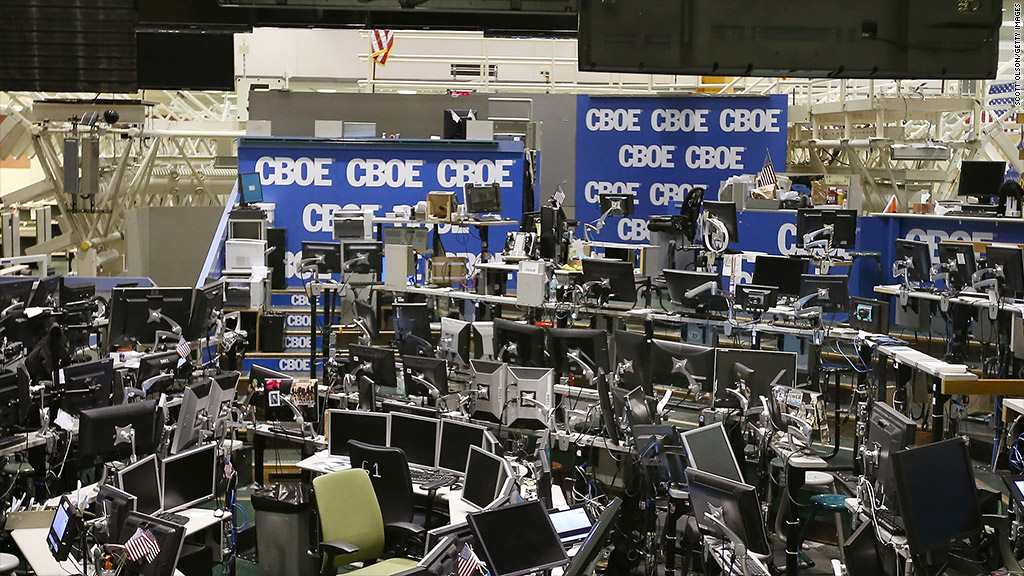
\includegraphics[width
		= 3cm]{ProgramsImages/130611131918-chicago-board-options-exchange-1024x576.jpg}}}
	
	\newcommand{\smallscoop}{\parbox{1cm}{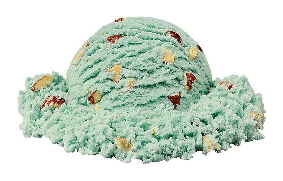
\includegraphics[width=1cm]{ProgramsImages/IceCreamScoop.eps}}\xspace}
	\newcommand{\medscoop}{\parbox{1.8cm}{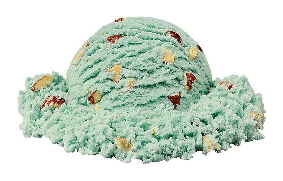
\includegraphics[width=1.8cm]{ProgramsImages/IceCreamScoop.eps}}\xspace}
	\newcommand{\meddanger}{\parbox{0.8cm}{\vspace{-0.3cm}\includegraphics[width=0.75cm]{ProgramsImages/dangersign.eps}}\xspace}
	\newcommand{\medcone}{\parbox{1.2cm}{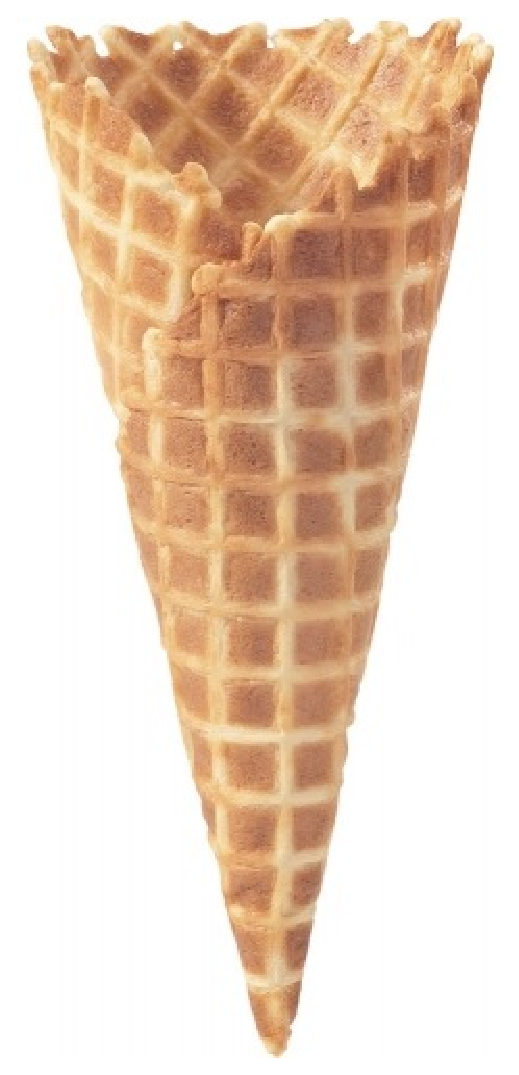
\includegraphics[width=0.55cm,angle=270]{ProgramsImages/MediumWaffleCone.eps}}\xspace}
	\newcommand{\largercone}{\parbox{2.2cm}{\vspace*{-0.2cm}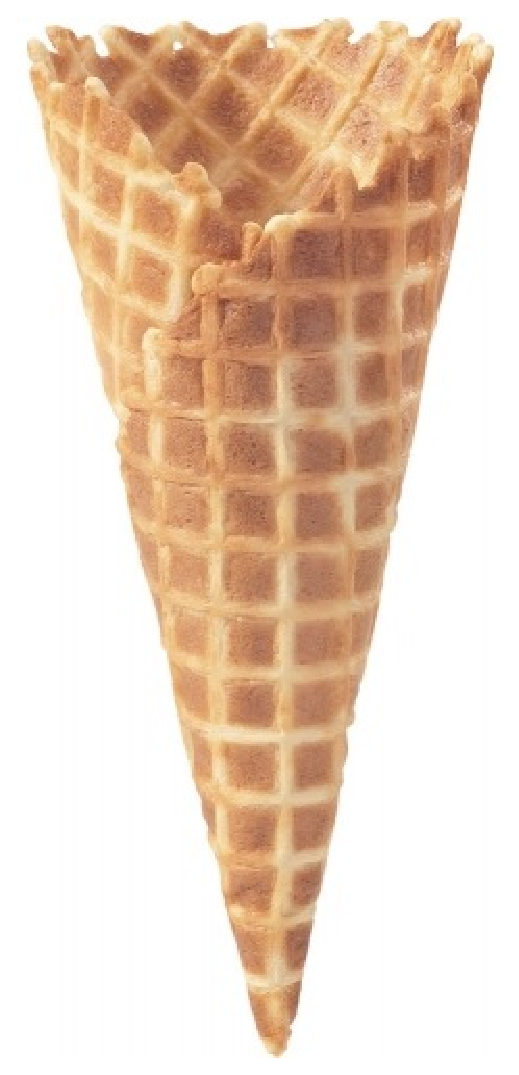
\includegraphics[width=1cm,angle=270]{ProgramsImages/MediumWaffleCone.eps}}\xspace}
	\newcommand{\largecone}{\parbox{1.54cm}{\vspace*{-0.2cm}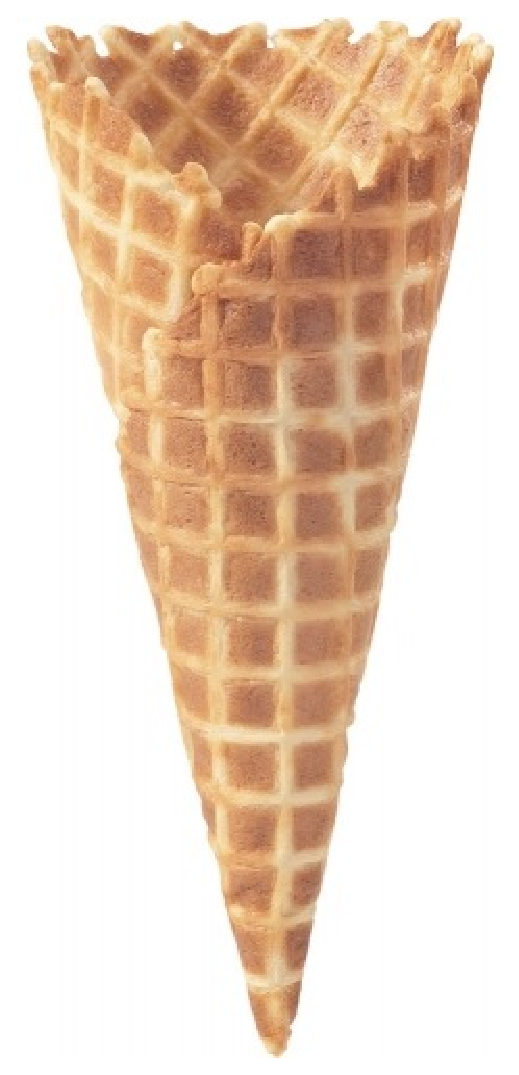
\includegraphics[width=0.7cm,angle=270]{ProgramsImages/MediumWaffleCone.eps}}\xspace}
	\newcommand{\smallcone}{\parbox{0.65cm}{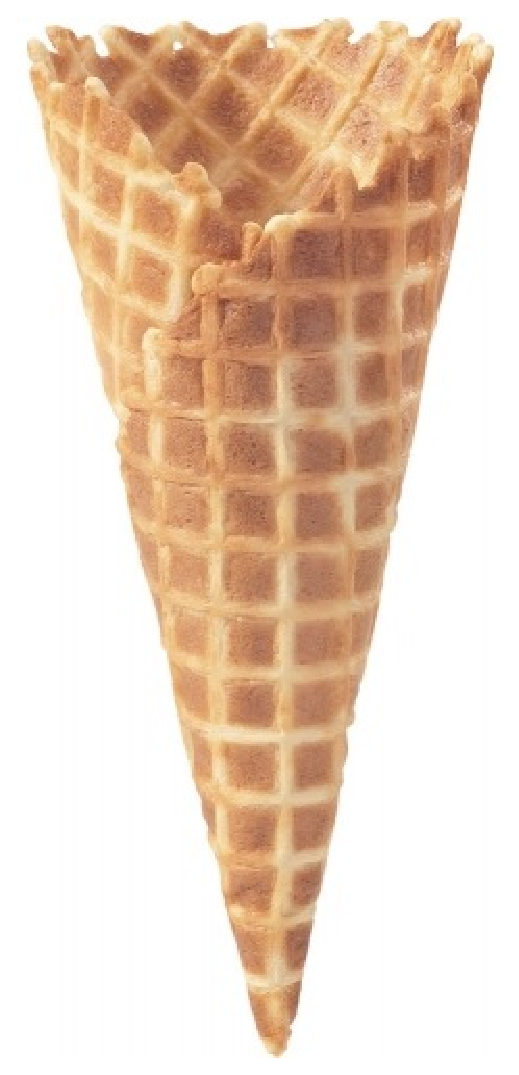
\includegraphics[width=0.3cm,angle=270]{ProgramsImages/MediumWaffleCone.eps}}\xspace}
	


\begin{document}
\everymath{\displaystyle}
\frame{\titlepage}
\section{Introduction}

\begin{frame}{Multivariate Linear Problems}
\vspace{-3ex}
\begin{tabular}{p{0.47\textwidth}p{0.5\textwidth}}
Given $f \in \cf$ find $g \in \cg$, where $g = \sol(f)$, \\
$\sol: \cf \to \cg$ is linear, e.g., 
\begin{gather*}
    g = \int_{\reals^d} f(\vx) \, \varrho(\vx) \, \dif \vx\\
    g = f\\
    g = \frac{\partial f}{\partial x_1} \\
    - \nabla^2 g = f, \ \  g = 0 \text{ on boundary}
\end{gather*}
&
\vspace{-10ex}
\begin{multline*}
    \ca(\ch) : = \{\app: \ch \times (0,\infty) \to \reals \text{ such that } \\
\norm[\cg]{\sol(f) - \app(f,\varepsilon) } \le \varepsilon \\ \forall f \in \ch \subseteq \cf, \ \varepsilon > 0 \}
\end{multline*}

\vspace{-2ex}
where $\app(f,\varepsilon)$ depends on \alert{function values}, \alert{Fourier coefficients}, or \alert{linear functionals}, e.g., 

\vspace{-4ex}
\begin{gather*}
    \app(f,\varepsilon) = \sum_{i=1}^n f(\vx_i) v_i, \quad v_i \in \cg \\
    \app(f,\varepsilon) = \sum_{i=1}^n \hf_i v_i, \quad v_i \in \cg \\
    \app(f,\varepsilon) = \sum_{i=1}^n L_i(f) v_i, \quad v_i \in \cg \\
\end{gather*}

\vspace{-4ex}
How big should $n$ be to satisfy error tolerance?

\end{tabular}
    
\end{frame}

\begin{frame}{Issues}

\vspace{-3ex}

\begin{tabular}{p{0.48\textwidth}p{0.49\textwidth}}
Given $f \in \cf$ find $g \in \cg$, where $g = \sol(f)$, \\
$\sol: \cf \to \cg$ is linear

\vspace{-2ex}

\begin{multline*}
    \ca(\ch) : = \{\app: \ch \times (0,\infty) \to \reals \text{ such that } \\
\norm[\cg]{\sol(f) - \app(f,\varepsilon) } \le \varepsilon \\ \forall f \in \ch \subseteq \cf, \ \varepsilon > 0 \}
\end{multline*}

\vspace{-2ex}
where $\app(f,\varepsilon)$ depends on \alert{function values}, \alert{Fourier coefficients}, or \alert{linear functionals}
&

\vspace{-9ex}
\uncover<2->{\alert{Solvability}\footfullcite{KunEtal19a}: $\ca(\ch) \ne \emptyset$

\medskip

\alert{Construction}: Identify concrete $\app \in \ca(\ch)$}

\medskip

\uncover<3->{\alert{Cost}: $\cost(\app,f,\varepsilon) = $ \# of function data
\newline
 $\cost(\app,\ch,\varepsilon, \rho) = \max_{f \in \ch \cap \cb_{\rho}} \cost(\app,f,\varepsilon)$
 \newline
 $\cb_{\rho} = \{f \in \cf : \norm[\cf]{f} \le \rho \}$
 
 \medskip

\alert{Complexity}\footfullcite{TraWasWoz88}: $\comp(\ca(\ch),\varepsilon,\rho)$ 
\newline \phantom{a} \hfill \hfill $= \min_{\app \in \ca(\ch)} \cost(\app,\ch,\varepsilon, \rho)$

\medskip

\alert{Optimality}:  \newline \phantom{a} \hfill \hfill $\cost(\app,\ch,\varepsilon, \rho) \le \comp(\ca(\ch),\alert{\omega} \varepsilon,\rho)$}

\medskip

\uncover<4->{\alert{Tractability}\footfullcite{NovWoz08a}: $\comp(\app,\ch,\varepsilon, \rho) \le C \rho^p\varepsilon^{-p} d^{q} $}

\vspace{-6ex}

\phantom{a}

\end{tabular}
    
\end{frame}

\thankyouframe

\printbibliography


\end{document}



\begin{frame}
\frametitle{What Does It Mean to Solve a Mathematics or Statistics Problem?}
\vspace{-5ex}

\[
\begin{array}{r@{\qquad}l}
	\text{Problem} & \text{Solution} \\
	\toprule
	x^2 +2 x - 3 = 0 &  x = -3, 1  \qquad \text{\alert{numbers}}\\
	\uncover<2->{\frac{\dif}{\dif x} \sin(x) & \cos(x) \qquad \text{\alert{elementary function}}} \\[2ex]
	\uncover<3->{\frac{1}{\sqrt{2\pi}} \int_{-\infty}^{1} \me^{-x^2/2} \, \dif x &  \Phi(1) \qquad \text{\alert{special function}} \\
	& \Phi \text{ is the standard Gaussian cumulative distribution function} } \\
\midrule
\uncover<4->{
\int_0^1 f(x) \, \dif x  & \text{Need a \alert{numerical solution}, i.e., } A(f,\varepsilon) \\[2ex]
f \text{ known via an algorithm} & \text{depending on integrand values } f(x_1), \, f(x_2), \ldots  \\
\text{i.e., can get } f(x) \ \forall x \in [0,1] & \text{such that } \abs{\int_0^1 f(x) \, \dif x - A(f,\varepsilon)} \le \varepsilon }
	\end{array}
	\]
\end{frame}

\begin{frame}
\frametitle{What About the Trapezoidal Rule?}
\vspace{-5ex}
\[
\int_0^1 f(x) \, \dif x \approx T_n(f)=\frac{1}{n}\left[\frac{f(0)}{2} + f\left(\frac{1}{n}\right) + \cdots + f\left(\frac{n-1}{n}\right) +  \frac{f(1)}{2} \right]
\]
\begin{tabular}{>{\raggedright}m{0.6\textwidth}@{\qquad}>{\centering}m{0.37\textwidth}}
\only<5->{\only<5-6>{Theory says
	\vspace{-3ex}
	\begin{equation*}
	\biggabs{\int_0^1 f(x) \, \dif x -T_n(f)} \le \frac{\overbrace{\int_0^1 \abs{f''(x)} \, \dif x}^{\text{curvature}}}{8 n^2} = \frac{\norm[1]{f''}}{8 n^2} \overset{\alert{?}}{\le} \varepsilon
	\end{equation*}
	
		\vspace{-1ex}
	\only<6>{Let $\cf = \{f :\norm[1]{f''} \le \rho \}$  \medscoop, and let}}\only<7->{Let}\uncover<6->{
	
	\vspace{-1ex}
	\[
	A(f,\varepsilon) = T_n(f) \quad \text{where }n = \left \lceil \sqrt{\frac{\rho}{8\varepsilon}} \, \right \rceil
	\]
	
	\vspace{-2ex}
	Then 
	\[
	 \abs{\int_0^1 f(x) \, \dif x - A(f,\varepsilon)} \le \varepsilon \quad \forall f \in \cf\only<7->{= \{f :\norm[1]{f''} \le \rho \}}, \, \varepsilon > 0
	 \]}}
	& 
	\only<1>{\includegraphics[width=5cm]{ProgramsImages/traprule-1.eps}\\$T_1(f)=0.5034$}
	\only<2>{\includegraphics[width=5cm]{ProgramsImages/traprule-2.eps}\\$T_2(f)=0.3949$}
	\only<3>{\includegraphics[width=5cm]{ProgramsImages/traprule-3.eps}\\$T_4(f)=0.3954$}
	\only<4->{\includegraphics[width=5cm]{ProgramsImages/traprule-4.eps}\\$T_{50}(f)=0.3957$}
\end{tabular}
\only<7->{We say that integration is \alert{solvable} for integrands in $\cf$  \medscoop}

\end{frame}

\section{Solvability}
\begin{frame}
\frametitle{Solvability\footfullcite{KunEtal19a}}
\vspace{-4ex}

A problem is called \alert{solvable} for a set of inputs $\cf$ \alert{if there exists} a numerical algorithm that provides a solution with error no greater than $\varepsilon$.  Specifically, integration is solvable for $\cf$ if there exists an $A$ for which 
	\[
\abs{\int_0^1 f(x) \, \dif x - A(f,\varepsilon)} \le \varepsilon \quad \forall f \in \cf, \, \varepsilon > 0
\]
\uncover<2->{We demonstrated that integration is solvable for 
\[
\cf = \{f :\norm[1]{f''} \le \rho \}  \quad \medscoop
\]
\uncover<3>{Is integration solvable for 
\[
\cf = \{f :\norm[1]{f''} < \alert{\infty} \} \quad \text{since } \biggabs{\int_0^1 f(x) \, \dif x -T_n(f)} \le  \frac{\norm[1]{f''}}{8 n^2} \alert{?}
\]
}}

\end{frame}

\begin{frame}
\frametitle{Integration Is \emph{Not} Solvable for $\cf = \{f :\norm[1]{f''} < \infty \}$}
\vspace{-3ex}
Suppose that there exists  $A$ such that 
\[
\abs{\int_0^1 f(x) \, \dif x - A(f,\varepsilon)} \le \varepsilon \quad \forall f \in \cf= \{f :\norm[1]{f''} < \infty \}, \, \varepsilon > 0
\]
\begin{tabular}{>{\raggedright}m{0.6\textwidth}@{\qquad}>{\centering}m{0.37\textwidth}}
	\begin{itemize}
	\item<2->Observe where $A(0,\varepsilon)$ gets function values
	
\item<3->Construct $f_{\text{bump}} \in \cf$, as tall as you like; note that $A(0,\varepsilon) = A(f_{\text{bump}},\varepsilon)$
	
	\item<4->  Since $\int_0^1 0 \, \dif x$ and $\int_0^1 f_{\text{bump}}(x) \, \dif x$ are so different, $A$ cannot be successful

\end{itemize}
	
	&
	\only<2>{\includegraphics[width=5cm]{ProgramsImages/ZeroFun.eps}}
	\only<3->{\includegraphics[width=5cm]{ProgramsImages/QuadHump.eps}}
\end{tabular}

\vspace{-5ex}

\uncover<5->{Why doesn't this argument hold for $\cf = \{f :\norm[1]{f''} \le \rho \}  \medscoop$? \\  \uncover<6->{Because $f_{\text{bump}} \notin \medscoop$}}

\end{frame}

\section{Optimality}

\begin{frame}
\frametitle{Is Trapezoidal Rule the Best Algorithm?}
\vspace{-4ex}
Let $\cost(A,f,\varepsilon)$ denote the number of function values, $n$ required for $A(f,\varepsilon)$ and 
\[
\cost(A,\cf,\varepsilon) = \sup_{f \in \cf} \cost(A,f,\varepsilon)
\]
For our trapezoidal rule algorithm, $A$
\[
\cost(A,\cf,\varepsilon) =  \cost(A,f,\varepsilon) = \left \lceil \sqrt{\frac{\rho}{8\varepsilon}} \right \rceil = \Order\left(\sqrt{ \frac{\rho}{\varepsilon}} \right) \qquad \forall f \in \cf = \{f :\norm[1]{f''} \le \rho \}  \medscoop
\]
This is the \alert{(up to a constant)} the smallest possible cost \uncover<2->{for integrands in $\cf = \{f :\norm[1]{f''} \le \rho \}  \medscoop$, no worse than Simpson's rule, Gauss rules, etc.}
\end{frame}

\finalthanksnote{Slides available on SpeakerDeck at
	\href{https://speakerdeck.com/fjhickernell/matrix-week-two-2018-june}
	{\nolinkurl{speakerdeck.com/fjhickernell/matrix-week-two-2018-june}}
}

\begin{frame}
\frametitle{Why the Trapezoidal Rule Is Optimal for $\cf = \{f :\norm[1]{f''} < \rho \}$}
\vspace{-3ex}
Let $A$ be \alert{any} algorithm satisfying
\[
\abs{\int_0^1 f(x) \, \dif x - A(f,\varepsilon)} \le \varepsilon \quad \forall f \in \cf= \{f :\norm[1]{f''} < \rho \}, \, \varepsilon > 0
\]

\vspace{-5ex}
\begin{tabular}{>{\raggedright}m{0.6\textwidth}@{\qquad}>{\centering}m{0.37\textwidth}}
	\begin{itemize}
		\item<2->Observe where $A(0,\varepsilon)$ gets function values
		
		\item<3->Construct $f_{\text{bump}} \in \cf$; note that $A(0,\varepsilon) = A(f_{\text{bump}},\varepsilon) = A(-f_{\text{bump}},\varepsilon)$
		
		\item<4->  For $A$ to succeed for $\pm f_{\text{bump}} $, which have different integrals, one must have 
		\[
		\cost(A,\cf,\varepsilon) =  \Order\left(\sqrt{ \frac{\rho}{\varepsilon}} \right)
		\]
		the same as the trapezoidal rule algorithm.
		
	\end{itemize}
	
	&
	\only<2>{\includegraphics[width=5cm]{ProgramsImages/ZeroFun.eps}}
	\only<3->{\includegraphics[width=5cm]{ProgramsImages/TwoQuadHump.eps}}
\end{tabular}

\vspace{-5ex}

\uncover<5->{Why do your instructors tell you that other algorithms are \alert{better than the trapezoidal rule}?  \\  \uncover<6->{They are only better when you assume that the integrand has \alert{more smoothness}}}

\end{frame}

\section{Adaptive Algorithms}

\begin{frame}
\frametitle{The Impracticality of Our Non-Adaptive Trapezoidal Rule Algorithm}
\vspace{-7ex}
\begin{tabular}{>{\raggedright}m{0.6\textwidth}@{\qquad}>{\centering}m{0.37\textwidth}}
\begin{gather*}
T_n(f)=\frac{1}{n}\left[\frac{f(0)}{2} + f\left(\frac{1}{n}\right) + \cdots + f\left(\frac{n-1}{n}\right) +  \frac{f(1)}{2} \right] \\
A(f,\varepsilon) = T_n(f) \quad \text{where }n = \left \lceil \sqrt{\frac{\rho}{8\varepsilon}} \, \right \rceil
\end{gather*}

\vspace{-2ex}
\begin{itemize}
	\item \alert{Solves} the integration problem for  $\cf = \{f :\norm[1]{f''} \le \rho \}$  \medscoop
	
	\item \alert{Costs} $\Order(\sqrt{\rho/\varepsilon})$ function values
	
	\item Is \alert{optimal} for $\cf = \{f :\norm[1]{f''} \le \rho \}$  \medscoop
\end{itemize}
	& 
	\includegraphics[width=5cm]{ProgramsImages/traprule-4.eps}\\$T_{50}(f)=0.3957$
\end{tabular}
What more could we want?

\uncover<2>{An algorithm that costs  $\Order(\sqrt{\norm[1]{f''}/\varepsilon})$  without needing to know  $\norm[1]{f''}$; \alert{cost depends on difficulty}}
\end{frame}

\begin{frame}
\frametitle{Adaptive Algorithms Don't Work for Balls, But May Work for Cones}
\vspace{-3ex}

\alert{Adptive} algorithms expend effort comensurate with the difficulty of the problem

\vspace{-3ex}
\begin{itemize}

	\item If $\cf = \medscoop$, then non-adaptive algorithms are optimal because $\medscoop$ is 
	\begin{description}
		
		\item[Balanced:] $f \in \cf \implies -f \in \cf$, and
		
		\item[Convex:] $f, g \in \cf \implies \theta \cf + (1 - \theta) g \in \cf$ for $0 \le \theta \le 1$
	
\end{description}

\end{itemize}

\vspace{-3ex}

\begin{tabular}{>{\raggedright}m{0.6\textwidth}@{\qquad}>{\centering}m{0.37\textwidth}}
	\begin{itemize}
		\item<2-> However, adaptive algorithms may be optimal for non-convex $\cf = \medcone$ ($f \in \cf \implies cf \in \cf$)
		
	\item<3-> We developed an adaptive trapezoidal rule that \alert{optimally solves} the integral for $\cf = \medcone$, a set of functions where the true curvature is not much more than its numerical approximation\footfullcite{HicEtal14b}
	
	\item<4-> Common adaptive algorithms in use \alert{have no theory}
	\end{itemize}
	& 
	\includegraphics[width=5cm]{ProgramsImages/traprule-4.eps}
\end{tabular}

\end{frame}

\begin{frame}
\frametitle{Adaptive Algorithms Don't Work for Balls, But May Work for Cones}
\vspace{-3ex}

We also developed adaptive algorithms for 

\vspace{-3ex}
\begin{itemize}
	
	\item Univariate integration by Simpson's rule\footfullcite{Zha18a} 
	
	\item Univariate function approximation and optimization\footfullcite{ChoEtal17a}

	\item Multivariate integration\footfullcite{HicEtal14a,HicJim16a,RatHic19a}
	
\end{itemize}

\vspace{-3ex} 

made available in the Guaranteed Automatic Integration Library (GAIL)\footfullcite{ChoEtal17b}


\end{frame}

\section{Open Problems}

\begin{frame}
\frametitle{Work to Be Done}

\vspace{-5ex}
\begin{itemize}
	
	\item Find $\cf = \medcone$ for which MATLAB's\footfullcite{MAT9.5} \alert{\mcode{integral_g}} or \alert{Chebfun}\footfullcite{TrefEtal17a} are guaranteed to solve the integration problem
	
	\item \alert{Locally} adaptive univariate integration
	
	\item Higher order \alert{function approximation}
	
	\item Adaptive \alert{multi-level Monte Carlo} methods\footfullcite{Gil15a}
	
	\item Adaptive multivariate \alert{function approximation}\footfullcite{DinHic20a}
	
	\item Other error criteria, such as \alert{relative error} or a hybrid of absolute and relative error\footfullcite{HicEtal17a}
	
	\item Combining our software efforts with that of other research groups
	
	
\end{itemize}


\end{frame}

\begin{frame}
\frametitle{Other Opportunities for You}

\begin{itemize}
	\item Join the Society for Industrial and Applied Mathematics (SIAM) for free \beamerbutton{\href{https://www.siam.org/Membership/Join-SIAM/Individual-Members/Student}{Click here}}
	
	\item Join the American Statististcal Association (ASA) for \$25 per year  \beamerbutton{\href{https://www.amstat.org/ASA/JoinRenew/JoinMemberType.aspx?membertype=IREG}{Click here}}
\end{itemize}
\end{frame}

\finalthanksnote{Slides available on SpeakerDeck at
	\href{https://speakerdeck.com/fjhickernell/can-we-solve-it-if-so-how-fast}
	{\nolinkurl{speakerdeck.com/fjhickernell/can-we-solve-it-if-so-how-fast}}
}


\thankyouframe

\printbibliography


\end{document}

